
\begin{frame}{A Frame with two Columns}
  % 
  \begin{columns}
    %
    \begin{column}{.45\textwidth}
      \minipage[c][0.65\textheight][s]{\columnwidth}
      
      On the left side text, figures on the right.

      \vfill

      \onslide<2->

      Start with basic figures, add more information later

      \vfill
      %\setlength{\abovedisplayskip}{0pt}
      \[\int_{0}^\infty f(x)\, dx = \frac{A}{B} = x^2 - \exp(\sqrt{x}) \]

      \vfill

      \onslide<3->

      Use \texttt{\textbackslash vfill} for the text column but not
      for figures.
 
      \vfill
      
      \begin{tabular}{|p{0.9\textwidth}}
        Use \texttt{minipage} for top aligned images, and
        \texttt{parbox} for vertically centered images.
      \end{tabular}

      
      \endminipage      
    \end{column}
    %
    \begin{column}{.55\textwidth}

      % for top aligned images use minipage
      \only<1-3>{
        \minipage[c][0.8\textheight][s]{\columnwidth}
        
        \onslide<1->    

        \only<1-3>{
          \begin{figure}
            \centering
            \includegraphics<1>[width=\textwidth]{%
              img/figure1.png} %
            \includegraphics<2-3>[width=\textwidth]{%
              img/figure1_red.png} %
        \end{figure}}
        
        \only<3>{
          \begin{figure}
            \centering
            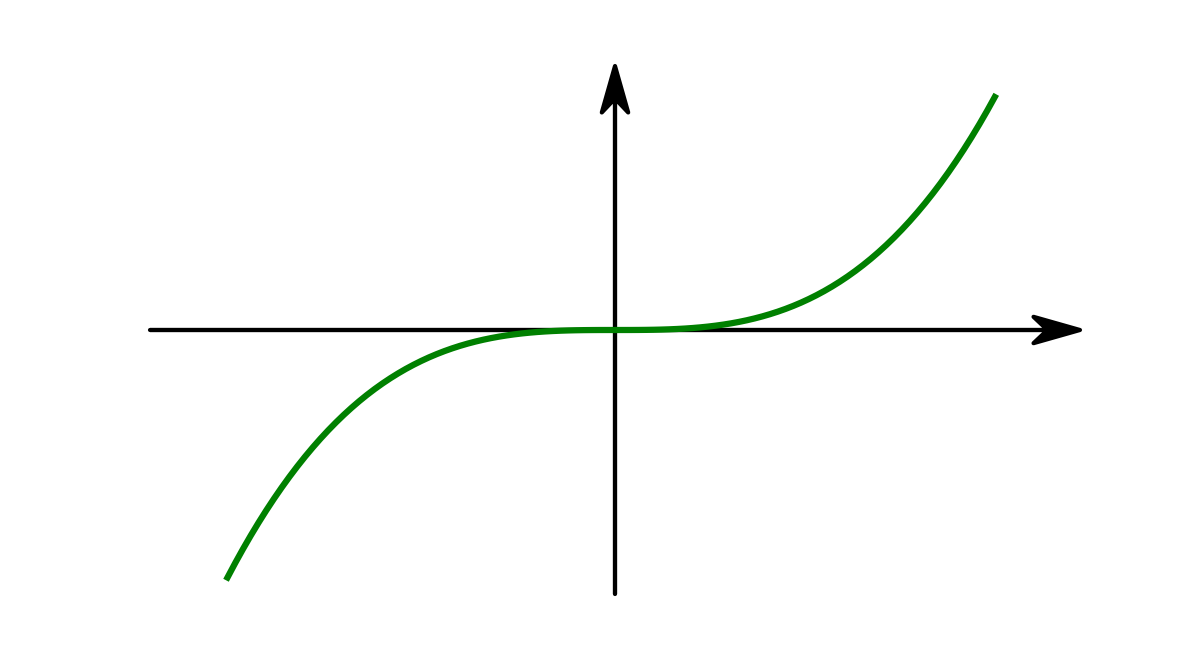
\includegraphics[width=\textwidth]{%
              img/figure2.png} %
        \end{figure}}
        
        \endminipage
      }   

      % for vertically centered images use parbox
      \only<4>{
        \parbox[c][0.8\textheight][c]{\columnwidth}{
          \begin{figure}
            \centering
            
\includegraphics[height=0.5\textheight]{%
              img/figure4.png} %
          \end{figure}
        }
      }

      \source{\cite{Hoffmann2015}}
      
    \end{column}
  \end{columns}

\end{frame}
